\documentclass{article}
%\usepackage[margin=1in]{geometry}
\usepackage{graphicx} % Required for inserting images
\usepackage{hyperref}
\usepackage{amsmath}
\usepackage{titling}
\usepackage{enumitem}
\usepackage{makecell}
\usepackage{minted}
 \usepackage{url}
\renewcommand\maketitlehooka{\null\mbox{}\vfill}
\renewcommand\maketitlehookd{\vfill\null}

\begin{document}
\title{\Huge Intro ML Homework 6}

\author{ \huge
Jaskin Kabir \\
\Large Student Id: 801186717 \\
\Large \href{https://github.com/jaskinkabir/Intro_ML/tree/main/HM6}{GitHub:}\\\url{https://github.com/jaskinkabir/Intro_ML/tree/main/HM6}
}

\date{November 2024}

\begin{titlingpage}
\maketitle
\end{titlingpage}

\section{Problem 1: Quadratic Temperature Conversion Model}
\begin{enumerate}[label=\alph*. ]
    \item{\textit{New Training Loop}}
    To accommodate the quadratic regression model, the forward function was modified to use a second weight for the square of the input temperature.
    \item{\textit{Training the Quadratic Model}}
    
    Using 5000 epochs for training, four different learning rates were used. The final loss values for these learning rates can be seen in Table \ref{tab:quad_loss} below.

    \begin{table}[htbp]
        \centering
        \begin{tabular}{|c|c|}
            \hline
            \textbf{Learning Rate} & \textbf{Final Loss} \\
            \hline
            1e-1 & 3.106353 \\
            \hline
            1e-2 & 3.832656 \\
            \hline
            1e-3 & 6.038405 \\
            \hline
            1e-4 & 3406753.75 \\
            \hline
        \end{tabular}
        \caption{Final Loss Values for Quadratic Model}
        \label{tab:quad_loss}
        
    \end{table}

    \item{\textit{Comparison to Linear Model}}
    
    The learning rate of 0.1 yielded the lowest loss, and was thus the most effective. Its loss value was 3.10653.

    With the same learning rate and number of epochs, the linear model was able to achieve an 8\% lower loss value of 2.92745. Thus, the linear model was more effective.

    This is also reflected in the plots of the linear and quadratic models' predictions, which can be seen in Figure \ref{fig:quad_vs_linear}.

    \begin{figure}[htbp]
        \centering
        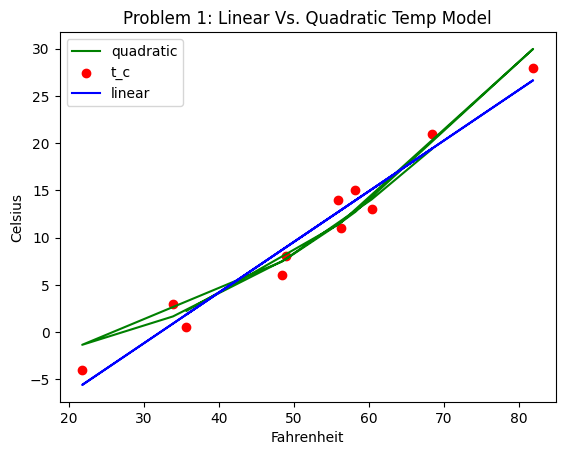
\includegraphics[width=0.6\textwidth]{images/im1.png}
        \caption{Quadratic vs. Linear Model Predictions}
        \label{fig:quad_vs_linear}
    \end{figure}
\end{enumerate}
\newpage
    \section{Problem 2: 5 Feature Housing Price Prediction}
    \begin{enumerate}[label=\alph*.]
        \item \textit{New Training Loop}
        To predict the housing price based on the five features provided, a model was developed as a class that inherits from the nn.Module class.
        
        \item \textit{Training the Model}
        To allow for a better comparison against the model trained in Homework 2, a custom MSE loss function was created that calculates the mean squared error of the predicted and actual prices and scales that loss based on the number of data points.

        Using 5000 training epochs, the model was trained with four different learning rates. The final loss values for these learning rates can be seen in Table \ref{tab:house_loss_1} below. For easier comparison with homework 2, which converted the final loss values to RMS, these loss values are also converted to RMS.
    
        \begin{table}[htbp]
            \centering
            \begin{tabular}{|c|c|}
                \hline
                \textbf{Learning Rate} & \textbf{Final Loss} \\
                \hline
                1e-1 & 3.54615E6 \\
                \hline
                1e-2 & 3.54668E6 \\
                \hline
                1e-3 & 3.54674E6 \\
                \hline
                1e-4 & 3.54674E6 \\
                \hline
            \end{tabular}
            \caption{Final RMS Loss Values for 5 Feature Housing Price Predictor}
            \label{tab:house_loss_1}
        \end{table}
    
        \item \textit{Comparison to Homework 2}
        With the handwritten gradient descent function from Homework 2, and the same parameters, the model was able to achieve an RMS loss of 8.934580e+05. This is 74\% lower than the best loss value achieved by the model trained in this homework assignment.
        
        It is unclear why the model trained in this assignment performed so poorly compared to the model trained in Homework 2. This may be due to the fact that the gradient descent function in Homework 2 calculates the gradient based on the mathematical derivation of the gradient of the loss function, while the model in this assignment uses PyTorch's built-in gradient calculation functions. PyTorch's gradient calculation in this case may not as accurate.
        
    
    \end{enumerate}

    \newpage
    \section{Problem 3: 11 Feature Housing Price Prediction}

    \begin{enumerate}[label=\alph*.]
        \item \textit{New Training Loop}
        The code written for the 5 feature housing price predictor already had the capability to accept an arbitrary number of features, so no modifications were made.
        \item \textit{Training the Model}
        The same training process was repeated, and the loss values for the four different learning rates can be seen in Table \ref{tab:house_loss_2} below.

        \begin{table}[htbp]
            \centering
            \begin{tabular}{|c|c|}
                \hline
                \textbf{Learning Rate} & \textbf{Final Loss} \\
                \hline
                1e-1 & 3.54592E6\\
                \hline
                1e-2 & 3.54666E6 \\
                \hline
                1e-3 & 3.54673E6 \\
                \hline
                1e-4 & 3.54674E6 \\
                \hline
            \end{tabular}
            \caption{Final RMS Loss Values for 11 Feature Housing Price Predictor}
            \label{tab:house_loss_2}
        \end{table}

        \item \textit{Comparison to Homework 2}
        Once again, the best model trained in this assignment performed much worse than the model trained in Homework 2. The loss of Homework 2's model was 7.602334e+05, which is 78\% lower than the best loss value achieved by the model trained in this assignment.

        The model trained on just 5 features performed only slightly worse than the model trained on all 11 features, which is different from Homework 2. In Homework 2, increasing the number of features resulted in a much more significant improvement in model performance.
         
    \end{enumerate}


\end{document}
